\documentclass[main.tex]{subfiles}
\begin{document}

\chapter{Examens}
\label{cha:examens}
In dit hoofstuk worden oude examens opgelost.
Er wordt telkens eerst de opgave gegeven en daarna de oplossing.
Merk op dat de opgaven gratis online beschikbaar zijn.
Let ook op, de examenvragen komen hoogstwaarschijnlijk niet terug, maar het zijn goede oefeningen.


\includepdf[pages=-]{opgaven/januari_2012_1.pdf}

\section{Januari 2012 I}

\subsection*{Mondeling gedeelte}
\begin{enumerate}
\item
  \begin{enumerate}[(a)]
  \item Zie definitie \ref{de:spiegeling} op pagina \pageref{de:spiegeling}
  \item Zie stelling \ref{st:spiegeling-isometrie} op pagina \pageref{st:spiegeling-isometrie}
  \item Een spiegeling om een $m$-dimensionale affiene deelruimte in een $n$-dimensionale affiene deelruimte is ori\"entatiebewarend als en slecht als $n+m$ even is.
    \begin{figure}[H]
      \centering
      \begin{tabular}{|c|c|c|c|c|}
        \hline
        Spiegeling om $\downarrow$ in $\rightarrow$& $0D$ & $1D$ & $2D$ & $3D$\\\hline\hline
        punt & Bewarend & Omkerend & Bewarend & Omkerend\\\hline
        rechte & N/A & Bewarend & Omkerend & Bewarend\\\hline
        vlak & N/A & N/A & Bewarend & Omkerend \\\hline
        ruimte & N/A & N/A & N/A & Bewarend\\\hline
      \end{tabular}
      \caption{Spiegelingen}
    \end{figure}
  \end{enumerate}
\item \TODO{}
\end{enumerate}
\subsection*{Schriftelijk gedeelte}
\begin{enumerate}
\item
  \begin{enumerate}[(a)]
  \item 
    \[
    \begin{pmatrix}
      2\\0\\1\\1
    \end{pmatrix}
    + \lambda
    \begin{pmatrix}
      1\\2\\0\\2
    \end{pmatrix}
    =
    \begin{pmatrix}
      -1\\0\\4\\-5
    \end{pmatrix}
    + \mu
    \begin{pmatrix}
      2\\0\\1\\2
    \end{pmatrix}
    \longleftrightarrow
    \begin{pmatrix}
      3\\0\\-3\\-4
    \end{pmatrix}
    =
    \lambda
    \begin{pmatrix}
      -1\\-2\\-0\\-2
    \end{pmatrix}
    + \mu
    \begin{pmatrix}
      2\\0\\1\\2
    \end{pmatrix}
    \]
    \[
    \left(
      \begin{array}{cc|c}
        -1 & 2 & 3\\
        2 & 0 & 0\\
        0 & 1 & -3\\
        -2 & 2 & -4
      \end{array}
    \right)
    \]
    Dit stelsel is strijdig, dus de doorsnede van $L_{1}$ en $L_{2}$ is leeg.
    $(1,2,0,2)$ is bovendien lineair onafhankelijk van $(2,0,1,2)$, dus de rechten kruisen.
  \item 
    We kennen de richting van de gemeenschappelijke loodlijn kennen we nu al, we berekenen dus nog het snijpunt ervan met $L_{1}$.
    \[ 
    \begin{pmatrix}
      2\\0\\1\\1
    \end{pmatrix}
    + a
    \begin{pmatrix}
      1\\2\\0\\2
    \end{pmatrix}
    =
    \begin{pmatrix}
      -1\\0\\4\\-5
    \end{pmatrix}
    + b
    \begin{pmatrix}
      2\\0\\1\\2
    \end{pmatrix}
    + c
    \begin{pmatrix}
      0\\1\\2\\-1
    \end{pmatrix}
    \longleftrightarrow
    \begin{pmatrix}
      2 & 0 & 1 & 3\\
      0 & 1 & 2 & 0\\
      1 & 2 & 0 & -3\\
      2 & -1 & 2 & 6
    \end{pmatrix}
    \]
    De oplossing hiervan is $(a,b,c)=(1,-2,1)$.
    Het snijpunt van $L_{1}$ met de gemeenschappelijke loodlijn is dus $p$:
    \[
    \begin{pmatrix}
      2\\0\\1\\1
    \end{pmatrix}
    +
    \begin{pmatrix}
      1\\2\\0\\2
    \end{pmatrix}
    =
    \begin{pmatrix}
      3\\2\\1\\3
    \end{pmatrix}
    \]
    De gemeenschappelijke loodlijn is dan $L_{3}$:
    \[
    L_{3} =
    \begin{pmatrix}
      3\\2\\1\\3
    \end{pmatrix}
    +
    \lambda
    \begin{pmatrix}
      0\\1\\2\\-1
    \end{pmatrix}
    \]
  \item Nee, de richtingsvector van de gemeenschappelijke loodlijn moet van een zeer specifieke vorm zijn.
    % Elke vector op de gemeenschappelijke loodlijn van $S$ en $T$ staat loodrecht op zowel $(1,2,0,2)$ als $(2,0,1,2)$:
    % \[
    % \left\{
    %   \begin{array}{c}
    %     (1,2,0,2) \cdot (u,x,y,z) = 0\\
    %     (2,0,1,2) \cdot (u,x,y,z) = 0
    %   \end{array}
    % \right.
    % \longleftrightarrow
    % \left\{
    %   \begin{array}{c}
    %     u+2x+2z = 0\\
    %     2u+y+z = 0
    %   \end{array}
    % \right.
    % \longleftrightarrow
    % \begin{pmatrix}
    %   1 & 0 & \frac{1}{2} & 1\\
    %   0 & 1 & -\frac{1}{2} & 1
    % \end{pmatrix}
    % \]
  \end{enumerate}

\item 
  \begin{figure}[H]
    \centering
    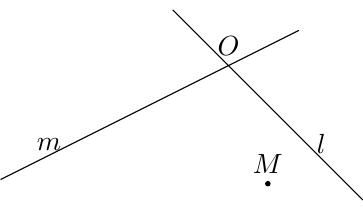
\begin{tikzpicture}[scale=1,extended line/.style={shorten >=-#1,shorten <=-#1},extended line/.default=1cm] 
      \coordinate [label=above:$O$] (o) at (1,2);
      \coordinate [label=left:$m$] (m1) at (-1,1);
      \coordinate [label=right:$l$] (l1) at (2,1);

      \draw [extended line=1cm] (o) -- (m1);
      \draw [extended line=1cm] (o) -- (l1);

      \coordinate [label=above:$M$] (m) at (1.5,.5);
      \fill (m) circle [radius=1pt];

    \end{tikzpicture}
  \end{figure}
  We zoeken een punt $A$ op $l$ en een punt $B$ op $m$ zodat $|AM|$ gelijk is aan $|MB|$ en $A$, $B$ en $M$ colineair zijn.
  Met andere woorden zodat $(A,B,M)$ gelijk is aan $1$.
  \[ M = \frac{1}{2}A + \frac{1}{2}B \]
  Noem het snijpunt van $l$ en $m$ $O$.
  \begin{itemize}
  \item Syntetisch\\
  \item \TODO{}
  \item Analytisch\\
  \item \TODO{}
  \item \TODO{}
  \end{itemize}
\item \TODO{}
\item 
  \begin{enumerate}[(a)]
  \item 
    \begin{itemize}
    \item $\beta$ is regulier: $\forall t:\ v_{\beta}(t) > 0$.
      \[ v_{\beta}(t) = \left\| \beta'(t) \right\| = \left\|\alpha'(t) + B'_{\alpha}(t) \right\| = \sqrt{\left\| \alpha'(t)\right\|^{2} + \left\| B'_{\alpha}(t) \right\|^{2}} = \sqrt{1 + \left\| B'_{\alpha}(t) \right\|^{2}} > 0\]
    \item $\beta$ heeft een constante snelheid als en slechs als $\tau_{\alpha}$ constant is:
      $\beta$ heeft een constante snelheid als en slechts als $B'_{\alpha}$ een constante lengte heeft.
      \[ B'_{\alpha} = -\tau_{\alpha}N_{\alpha} \]
      \[ \left\|B'_{\alpha}\right\| = \left\|\tau_{\alpha}N_{\alpha}\right\| = \tau_{\alpha} \left\|N_{\alpha}\right\| \]
      Hierin is $\left\|N_{\alpha}\right\|$ identiek $1$. $\left\|B'_{\alpha}\right\|$ is dus constant als en slechts als $\tau_{\alpha}$ constant is.
    \end{itemize}
  \item 
    Een cirkelschroeflijn heeft een constante torsie en kromming.
    Stel dat $\alpha$ een cirkelschroeflijn is:
    \[ \kappa_{\alpha}(t) = \kappa_{\alpha} \quad \tau_{\alpha}(t) = \tau_{\alpha} \]
    We weten uit (a) al dat $\beta$ een constante snelheid zal hebben.
    \[ v_{\beta} = \sqrt{1-\tau_{\alpha}^{2}}\]
\TODO{}
\item 
\TODO{}
  \end{enumerate}
\end{enumerate}


\includepdf[pages=-]{opgaven/januari_2012_2.pdf}

\section{Januari 2012 II}
\subsection*{Mondeling gedeelte}
\begin{enumerate}
\item Zie stelling \ref{st:vaste-punten-deelruimte} op pagina \pageref{st:vaste-punten-deelruimte} en eigenschap \ref{ei:dim-vaste-punten-even} op pagina \pageref{ei:dim-vaste-punten-even}.
\item Zie stelling \ref{st:congruentiestelling-ruimtekrommen} op pagina \pageref{st:congruentiestelling-ruimtekrommen}.
\end{enumerate}
\subsection*{Schriftelijk gedeelte}
\begin{enumerate}
\item 
  \begin{enumerate}[(a)]
  \item
    We bepalen eerst de doorsnede van $l$ en $\pi$:
    \[
    l \cap \pi \leftrightarrow
    \left\{
    \begin{array}{c}
      2(2+\mu) + (1+\mu) + (2+\mu) = 2\\
      (0) - 2(2+\mu) = 1
    \end{array}
    \right.
    \leftrightarrow
    \left\{
      \begin{array}{rl}
        4\mu+5 &= 0\\
        -2\mu-5 &= 0
      \end{array}
    \right.
    \]
    Dit stelsel is strijdig, dus de doorsnede is leeg.
    We berekenen nu de parametervergelijkingen van $\pi$ om daarna de evenwijdigheid te onderzoeken:
    \[ 
    \left(
      \begin{array}{cccc|c}
        2 & 0 & 1 & 1 & 2\\
        0 & 1 & 0 & -2 & 1
      \end{array}
    \right)
    \rightarrow
    \left(
      \begin{array}{cccc|c}
        1 & 0 & \frac{1}{2} & \frac{1}{2} & 1\\
        0 & 1 & 0 & -2 & 1
      \end{array}
    \right)
    \]
    \[ \pi \leftrightarrow 
    \begin{pmatrix}
      -1\\ -1\\ 0\\ 0\\
    \end{pmatrix}
    +\lambda
    \begin{pmatrix}
      -1\\0\\2\\0\\
    \end{pmatrix}
    +\mu
    \begin{pmatrix}
      -1\\ 4\\ 0\\ 1
    \end{pmatrix}
    \]
    We zien dat de richting van $l$ lineair onafhankelijk is van de richting van $\pi$, dus ze kruisen.
  \item 
    We zoeken eerst de euclidische deelruimte $S$ door $(2,1,-2,0)$ die orthogonaal is met $l$.
    Noem $V$ de richting van $l$:
    \[
    V^{\bot} \leftrightarrow
    \left\{
    x_{1} + x_{3} + x_{4} = 0
    \right.
    \leftrightarrow
    \left(
      \begin{array}{cccc|c}
        1 & 0 & 1 & 1 & 0\\
      \end{array}
    \right)
    =
    \{ (-\mu -\nu, \lambda,\mu,\nu) \mid \lambda,\mu,\nu \in \mathbb{R} \}
    \]
    $S$ ziet er dan als volgt uit:
    \[ S  = 
    \begin{pmatrix}
      2\\1\\-2\\0
    \end{pmatrix}
    +
    \lambda
    \begin{pmatrix}
      0\\1\\0\\0
    \end{pmatrix}
    + \mu
    \begin{pmatrix}
      -1\\0\\1\\0
    \end{pmatrix}
    + \nu
    \begin{pmatrix}
      -1\\0\\0\\1
    \end{pmatrix}
    \]
    Tenslotte zoeken we de doorsnede van $\pi$ en $S$, dit is dan de gezochte rechte:
    \[
    \pi\cap S \leftrightarrow
    \left\{
      \begin{array}{c}
        2(2-\mu-\nu) + (-2+\mu) + (\nu) = 2\\
        (1-\lambda)-2(\nu) = 1
      \end{array}
    \right.
    \leftrightarrow
    \left\{
      \begin{array}{rl}
        -\mu -\nu&=0\\
        \lambda-2\nu&=0
      \end{array}
    \right.
    \leftrightarrow
    \left(
      \begin{array}{ccc|c}
        0 & -1 & -1 & 0\\
        1 & 0 & -2 & 0
      \end{array}
    \right)
    \]
    \[
    \leftrightarrow
    \left(
      \begin{array}{ccc|c}
        1 & 0 & -2 & 0\\
        0 & 1 & 1 & 0
      \end{array}
    \right)
    \leftrightarrow (\lambda,\mu,\nu) \in \{ (2t,-t,t) \mid t\in \mathbb{R} \}
    \]
    \[
    \pi\cap S \leftrightarrow
    \begin{pmatrix}
      2\\1\\-2\\0
    \end{pmatrix}
    +2t
    \begin{pmatrix}
      0\\1\\0\\0
    \end{pmatrix}
    -t
    \begin{pmatrix}
      -1\\0\\1\\0
    \end{pmatrix}
    +t
    \begin{pmatrix}
      -1\\0\\0\\1
    \end{pmatrix}
    = 
    \begin{pmatrix}
      2\\1\\-2\\0
    \end{pmatrix}
    +t
    \begin{pmatrix}
      0\\2\\-1\\1
    \end{pmatrix}
    \]
  \end{enumerate}
\item
  We antwoorden eerst op vraag (b) omdat dat ons toelaat om (a) makkelijker te beantwoorden.
  Zie gevolg \ref{gev:verhouding-volumes-affien-invariant} op pagina \pageref{gev:verhouding-volumes-affien-invariant}.
  De verhouding tussen de oppervlakken zijn affien invariant, dus ook of die al dan niet groter is dan $1$.
  We zetten daarom de situatie om naar de volgende met de unieke\gevref{gev:affiene-invariante-punten-transformatie} affiene transformatie die de affien onafhankelijke punten $A$, $B$ en $C$ afbeeldt op respectievelijk $(0,0)$, $(2,0)$ en $(0,2)$.

  \begin{figure}[H]
    \centering
    \begin{tikzpicture}[scale=2,extended line/.style={shorten >=-#1},extended line/.default=1cm] 
      \coordinate [label=left:$A$] (a) at (0,0);
      \coordinate [label=below:$B$] (b) at (2,0);
      \coordinate [label=left:$C$] (c) at (0,2);

      \draw [extended line=2.5cm] (a) -- (b);
      \draw [extended line=.5cm] (a) -- (c);

      \coordinate [label=above:$M$] (m) at ($(b)!.5!(c)$);
      \fill (a) circle [radius=1pt];
      \fill (b) circle [radius=1pt];
      \fill (c) circle [radius=1pt];
      \fill (m) circle [radius=1pt];
      \draw [dashed] (c) -- (m) -- (b);
      
      \filldraw[fill=blue,opacity=.2] (a)
        to (b)
        to (c);

      \coordinate [label=below:$B'$] (bp) at (3,0);
      \coordinate [label=left:$C'$] (cp) at (0,1.5);
      \fill (bp) circle [radius=.5pt];
      \fill (cp) circle [radius=.5pt];
      \draw [dashed] (cp) -- (m) -- (bp);
      
      \filldraw[fill=red,opacity=.2] (a)
        to (bp)
        to (cp);

    \end{tikzpicture}
    \caption{De situatie na du affiene transformatie}
  \end{figure}

  We zullen nu bewijzen dat de blauw gearceerde oppervlakte $\mathcal{O}$ minimaal is steeds kleiner is dan de rood gearceerde oppervlakte.
  Kies immers een punt $B'$ op $AB$, dan moet $B'$ coordinaten $(x,0)$ hebben voor een bepaalde $x\in \mathbb{R}$.
  $C'=(0,y)$ ligt dan op $m'=B'M$:...
  \[ m' \leftrightarrow (x,0) + \lambda(1-x,1) \]
  ... maar ook op $AC$:
  \[ (0,y) = (x,0) + \lambda (1-x,1) \]
  $C$ heeft dus $(0,\frac{x}{1-x})$ als co\"ordinaten. 
  De oppervlakte $\mathcal{O}'$ is dan als volgt:
  \[ \mathcal{O}' = \frac{1}{2} \cdot x \cdot \frac{x}{1-x} = \frac{x^{2}}{2(1-x)} \]
  Er rest ons dus nog te bewijzen dat dit groter of gelijk is aan $2$.
  \[ \frac{x^{2}}{2(1-x)} \ge 2 \Leftrightarrow \frac{x^{2}}{1-x} \ge 4 \Leftrightarrow x^{2}+4x-4 \ge 0 \Leftrightarrow (x-2)^{2} \ge 0 \]
  $\mathcal{O}'$ is dus groter dan of gelijk aan $\mathcal{O}$ met een gelijkheid wanneer $B'$ gelijk is aan $B$ (en dus $C'$ ook gelijk aan $C$).

\item
  \begin{enumerate}[(a)]
  \item 
    Een dilatatie is een affiene transformatie van de vorm $F$:
    \[ F:\ p \mapsto \lambda Ip+b \] We bewijzen nu dat $F$ hoeken
    bewaart of (, nog straffer), het volgende:
    \[
    \forall v,w \in T_{p}\mathbb{E}:\
    \frac{\left\|F(v)\right\|\left\|F(w)\right\|}{F(v) \cdot F(w)} =
    \frac{\lambda\left\|v\right\|\lambda\left\|w\right\|}{\lambda^{2}(v\cdot
      w)} = \frac{\left\|v\right\|\left\|w\right\|}{v\cdot w}
    \]
    Er geldt immers het volgende:
    \[
    \forall v \in T_{p}\mathbb{E}:\
    \begin{array}{rll}
      \left\|F(v)\right\| &= \sqrt{ (\lambda v_{1})^{2} + \dotsb + (\lambda v_{n})^{2} }\\
      &= \sqrt{ \lambda^{2} (v_{1}^{2} + \dotsb + v_{n}^{2}) } &= \lambda \left\|v\right\|
    \end{array}
    \]
    \[
    \forall v,w \in T_{p}\mathbb{E}:\
    \begin{array}{rll}
      F(v)\cdot F(w)  &= \sum_{i=1}^{n}(\lambda v_{i})(\lambda w_{i})\\
      &= \lambda^{2} \sum_{i=1}^{n} v_{i}w_{i} &= \lambda^{2}(v\cdot w)
    \end{array}
    \]
  \item 
    \TODO{}
  \item 
    Een cilinderschroeflijn is gedefinieert als een curve die overal dezelfde hoek maakt met een bepaalde vector.
    Omdat dilataties volgens (a) hoeken behouden behouden dilataties ook het cilinderschroeflijn-zijn.
  \end{enumerate}

\item 
\TODO


\end{enumerate}





%\includepdf[pages=-]{opgaven/januari_2011_1.pdf}
%\includepdf[pages=-]{opgaven/januari_2011_2.pdf}
%\includepdf[pages=-]{opgaven/augustus_2011.pdf}
%\includepdf[pages=-]{opgaven/januari_2009_2.pdf}

\end{document}
